%!TEX root = fp.tex

% Author: Philipp Moers <soziflip funny character gmail dot com>

\chapter{Values and Types} % (fold)
\label{cha:values_and_types}

Any Haskell expression e has a type t (\codeline{e :: t}) that is determined at compile time.
The \textbf{type assigmnent ::} is either given explicitly or inferred by the compiler.


\section{Base Types}

\vspace{9pt}\begin{center}\begin{tabular}{|c|c|c|}\hline
\rowcolor{grau}     Type            & Description                                   & values                                \\\hline
                    Int             & fixed-prec. integer                           & 0, 1, (-42)                           \\\hline
                    Integer         & arbitrary prec. integer                       & 10\textasciicircum 100                \\\hline
                    Float, Double   & single/double floating point (IEEE)           & 0.1, 1e02                             \\\hline
                    Char            & Unicode character                             & ``x'', ``\textbackslash t'', 
                                                                                        ``$\triangle$'', ``\textbackslash 8710''\\\hline
                    Bool            & Boolean                                       & True, False                           \\\hline
                    ()              & Unit                                          & ()                                    \\\hline
\end{tabular}\end{center}\vspace{9pt}


\section{Type Constructors}

\begin{itemize}
    \item Build new types from existing types
    \item Let a, b \dots denote arbitrary types (\textbf{type variables})
\end{itemize}

\vspace{9pt}\begin{center}\begin{tabular}{|c|c|c|}\hline
\rowcolor{grau}     Type            & Description                                   & values                        \\\hline
                    (a, b)          & pairs of values of type a, b                  & (1, True) :: (Int, Bool)      \\\hline
                    (a$_1$, a$_2$, \dots a$_n$) & n-tuples                          &                               \\\hline
                    [a]             & list of values of type a                      & [True, False] :: [Bool], []::[a]          \\\hline
                    Maybe a         & optional value of type a                      & \multirow{2}{3.7cm}{Just 42 :: Maybe Int 
                                                                                                         Nothing :: Maybe a}    \\
                                    &                                               &                               \\\hline
                    Either a b      & choice                                        & \multirow{2}{5cm}{Left ``x'' :: Either Char b
                                                                                                     Right pi :: Either a Double}   \\
                                    &                                               &                               \\\hline
                    IO a            & \multirow{2}{4.2cm}{I/O actions that 
                                                            return a value of type a}   & print 42 :: IO ()             \\
                                    &                                               &                               \\\hline
                    a ->\ b& functions from a to b                       & isLetter :: Char ->\ Bool      \\\hline
\end{tabular}\end{center}\vspace{9pt}


\section{Currying}

\begin{itemize}
  \item \textit{Recall}: \codeline{e$_1$ ++ e$_2$} $\equiv$ \codeline{(++) e$_1$ e$_2$}
  \item \codeline{(++) e$_1$ e$_2$} $\equiv$ \codeline{((++) e$_1$) e$_2$}
  \item Function application happens one argument at a time. \\ (\textbf{Currying}, Haskell B. Curry)
  \item Type of n-ary function is \\ a$_1$ -> a$_2$ -> \dots a$_n$ -> b
  \item Type fun -> associates to the right, read above type as \\ a$_1$ -> (a$_2$ -> (\dots ($a_n$ -> $b$)))
  \item Enables \textbf{Partial Application}
\end{itemize}


\section{Defining Values (and thus functions)}

\begin{itemize}
  \item \codeline{=} binds names to values. Names must not start with A-Z (Haskell style: camelCase)
  \item Define constant (0-ary function) c. Value of c is value of expression e. \\ \codeline{c = e}
  \item Define n-ary function f with arguments x$_i$. f may occur in e. \\ \codeline{f x$_1$ x$_2$ \dots x$_n$ = e}
  \item A Haskell program is a set of bindings.
  \item Good style: give type assigmnents for top-level (global) bindings: 
  \begin{codebox}[haskell]
f :: a@$_1$@ -> a@$_2$@ -> b
f x@$_1$@ x@$_2$@ = e
  \end{codebox}
\end{itemize}

\subsection{Guards}

Guards are conditional expressions (something like ``switch'' in Java).
They are a lot more readable and more powerful than \codeline{if \dots then \dots else \dots}.

Guards are introduced by \codeline{|}:
\begin{codebox}[haskell]
f x@$_1$@ x@$_2$@ @\dots@ x@$_n$@
  | q@$_1$@     = e@$_1$@
  | q@$_2$@     = e@$_2$@
  @\dots@
  | q@$_m$@     = e@$_m$@
[ | otherwise   = e@$_{m+1}$@ ]
\end{codebox}

Guards (q$_i$) are expressions of type Bool, evaluated top to bottom.

\codefile{haskell}{caption={factorial.hs}, label=factorial.hs}{../material/factorial.hs}



\subsection{Local Definitions}

\begin{enumerate}
  \item \textbf{Where bindings}: local definitions visible in the entire rhs of a definition.\\
  \begin{codebox}[haskell]
f@$_1$@ x@$_1$@ x@$_2$@ @\dots@ x@$_n$@ | q@$_1$@ = e@$_1$@
                    | q@$_2$@ = e@$_2$@ 
                    @\dots@
                    | q@$_m$@ = e@$_m$@ 
          where 
              g@$_1$@ = @\dots@
              g@$_2$@ = @\dots@
              @\dots@
              g@$_o$@
  \end{codebox}

  \codefile{haskell}{caption={power.hs}, label=power.hs}{../material/power.hs}

  \item \textbf{Let expressions}: local definitions visible inside one expression.\\
  \begin{codebox}[haskell]
let g@$_1$@ = @\dots@
    g@$_2$@ = @\dots@
    @\dots@
    g@$_o$@
in e
  \end{codebox}
\end{enumerate}


\subsection{Lists}

\begin{itemize}
  \item Recursive definitions:
  \begin{enumerate}
      \item \codeline{[]} is a list (nil), type [] :: [a]
      \item \codeline{x:xs} is a list, if x :: a, xs :: [a] \\ (x is head, xs is tail)
  \end{enumerate}
  \item Notation: \codeline{3:(2:(1:[]))} $\equiv$ \codeline{3:2:1:[]} $\equiv$ \codeline{[3,2,1]} $\equiv$ \codeline{3:[2,1]}
  \item Law: $\forall$ xs :: [a] :   \hspace{1cm} (xs $\neq$ []) \\
      \codeline{head xs : tail xs} == xs
\end{itemize}




\subsection{Pattern Matching}

\begin{itemize}
  \item \textit{The} idiomatic Haskell way to define a function by cases:
  \begin{codebox}[haskell]
f :: a@$_1$@ -> @\dots@ a@$_n$@ -> b
f p@$_11$@ @\dots@ p@$_1k$@ = e@$_1$@
f p@$_21$@ @\dots@ p@$_2k$@ = e@$_2$@
@\dots@
f p@$_n1$@ @\dots@ p@$_nk$@ = e@$_k$@
  \end{codebox}

\end{itemize}

\vspace{9pt}\begin{center}\begin{tabular}{|c|c|c|}\hline
\rowcolor{grau}   Pattern         & Matches If                & Bindings in e$_r$     \\\hline
                  constant c      & x$_i$ == c                  &                     \\\hline
                  variable v      & always                    & v $\equiv$ x$_i$      \\\hline
                  wildcard \_      & always                    &                       \\\hline
                  tuple (p$_1$, \dots p$_m$)  & components of x$_i$ match patterns p    & \\\hline
                  []              & x$_i$ == []                 &                     \\\hline
                  (p$_1$ : p$_2$)     & head x$_i$ matches p$_1$, tail x$_i$ matches p$_2$    & \\\hline
\end{tabular}\end{center}\vspace{9pt}


\codefile{haskell}{caption={tally.hs}, label=tally.hs}{../material/tally.hs}
\newpage
\codefile{haskell}{caption={take.hs}, label=take.hs}{../material/take.hs}
\codefile{haskell}{caption={mergesort.hs}, label=mergesort.hs}{../material/mergesort.hs}




\section{Algebraic Data Types}

(also known as \textbf{Sum-of-Product-Types})

\begin{itemize}
  \item \textit{Recall}: \codeline{[]} and \codeline{(:)} are the \textbf{values constructors} for \textbf{type constructor} [a]. 
  \item Can define entirely new type T and its constructors K$_i$:
        \begin{codebox}[haskell]
data T a@$_1$@ a@$_2$@ @\dots@ a@$_n$@ = K@$_1$@ b@$_{11}$@ @\dots@ b@$_{1_{n_1}}$@
                     K@$_2$@ b@$_{21}$@ @\dots@ b@$_{2_{n_2}}$@
                     @\dots@
                     K@$_r$@ b@$_{r1}$@ @\dots@ b@$_{r_{n_r}}$@
        \end{codebox}
        b$_{ij}$ types mentioning the type vars a$_1$ \dots a$_n$

  \item Defines type constructor T and r value constructors:\\
        \codeline{K$_i$ :: b$_{i_1}$ -> b$_{i_2}$ -> \dots b$_{in_i}$ -> T a$_1$ \dots a$_n$}
  \item Compare \codeline{[] :: [a]} and \codeline{(:) :: a -> [a] -> [a]}
  \item \textbf{Sum Type} (n=0, n$_i$ = 0) 
        \codefile{haskell}{caption={weekday.hs}, label=weekday.hs}{../material/weekday.hs}
  \item Add \codeline{deriving (c, c, \dots c)} to data declaration to define canonical operations: 
  \vspace{9pt}\begin{center}\begin{tabular}{|c|c|}\hline
  \rowcolor{grau} c       & operations                          \\\hline
                  Eq      & equality (==, /=)                   \\\hline
                  Show    & printing (show)                     \\\hline
                  Ord     & ordering (<, <=, max)               \\\hline
                  Enum    & enumeration                         \\\hline
                  Bounded & minBound, maxBound                  \\\hline
  \end{tabular}\end{center}\vspace{9pt}
  % \codefile{haskell}{caption={deriving.hs}, label=deriving.hs}{../material/deriving.hs}
  \item \textbf{Product Types} (r=1)
  \codefile{haskell}{caption={sequence.hs}, label=sequence.hs}{../material/sequence.hs}
  \item \textbf{Sum-of-Product-Types}\\
    \codeline{data Maybe a = Just a | Nothing}\\
    \codeline{data Either a b = Left a | Right b}\\
    \codeline{data List a = Nil | Cons a (List a)}
    \codefile{haskell}{caption={cons.hs}, label=cons.hs}{../material/cons.hs}
    \textit{Anschauung zu liftList:}
    % List a  - fromList ->   [a]
    % | g                     ^ 
    % v                       | g''
    % List b  - toList  ->    [b]
    \begin{center} 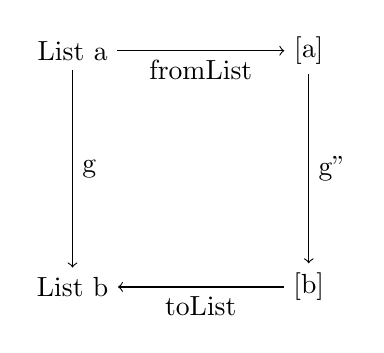
\begin{tikzpicture}[node distance = 3cm]
      \node                     (lista) {List a};
      \node [below of = lista]   (listb) {List b};
      \node [right of = lista]   (la) {[a]};
      \node [right of = listb]   (lb) {[b]};
      \path[->] (lista) edge[right] node[below] {fromList} (la)
                (lb) edge[right] node[below] {toList} (listb)
                (lista) edge[below] node[right] {g} (listb)
                (la) edge[below] node[right] {g''} (lb)
      ;
    \end{tikzpicture} \end{center}

  \codefile{haskell}{caption={eval-compile-run.hs}, label=eval-compile-run.hs}{../material/eval-compile-run.hs}
  \item \textit{Erläuterung zur Super-simple stack machine}:\\
    \begin{itemize}
      \item ``push'' pushes a new element to the stack
      \item ``DoAdd'' substitutes the first two elements of the stack with their sum
    \end{itemize}

        
\end{itemize}





% chapter values_and_types (end)




